% !TeX root = ../build/main.tex

\martai{Is the process called voting? Election, poll?}

\subsection{Parties involved}
\label{sec:vocdoni-protocol:parties}

A voting process involves three types of participants: the organizer, the sequencer, and the voters.

\paragraph{Organizer.} The organizer is the entity responsible for defining and setting up the voting process. Its key responsibilities include defining the voting parameters and gathering the census data. The organizer ensures that the election is structured correctly but does not participate in vote collection or tallying.

\paragraph{Sequencer.} Sequencers are a set of decentralized parties that facilitate the voting process. On the one hand, they collaboratively generate a public encryption key that voters use to encrypt their votes. Then, during the voting phase, they receive and verify encrypted votes from voters and reencrypt votes to prevent coercion.
 
\paragraph{Voter.} Voters are the participants that belong the census that cast their votes in the election. 

\subsection{Components}
\label{sec:vocdoni-protocol:components}

\subsubsection{Merkle trees} 

\textit{Old text: Merkle trees are employed to create a cryptographic representation of both the voter registry (census) and the voting process state:
	\begin{itemize}
		\item \textbf{Census}: Each voter is assigned a Merkle proof, which they use to prove their eligibility to vote. This mechanism ensures efficient and secure verification of voter eligibility.
		\item \textbf{State}: The voting process state is represented as a Merkle tree, with new votes being added to the tree. The root of this Merkle tree is stored on Ethereum, allowing multiple sequencers to participate in the voting phase and ensuring consistency. 
\end{itemize}}

\paragraph{Census Merkle tree.} Explain what it is. \\

\martai{There is a whole section about the Census Merkle tree in the whitepaper -- CHECK!!}

\martai{It could actually be another type of data structure. We only need to be able to get a commitment and a membership proof that can be proven in-circuit. Mention it in some way.}

\martai{One way to think about it: (weight, pk).}

\paragraph{State Merkle tree.} Explain what it is and the structure. Below, the original text:\\

\martai{Essentially, the first "addresses" or "leaves" are reserved to those items (like processId, censusRoot, etc.), and then the voters' addresses and nullifiers are used as paths to the leave where the encrypted ballot/commitment is stored.}

The State tree contains some special addresses (indices) for storing some required data regarding the voting process:

\begin{itemize}
	\item Address \texttt{0x0}: it stores \processid, a unique identifier for the voting process.
	\item Address \texttt{0x1}: it stores \censusroot and \type, which contains the necessary information to validate vote proofs.
	\martai{they type was a field in case the organization was using a different structure for the census than a MT.}
	\item Address \texttt{0x2}: it stores \ballotmode, which encodes rules for validating votes, such as the maximum number of selectable options.
	\item Address \texttt{0x3}: it stores the \epk, which is the public key used to encrypt the votes.
	\martai{Ideally, EPK is computed before the organization sets the tree, but I am not sure how practical this is.}
	\item Address \texttt{0x4}: it stores the \addaccumulator. That is, the aggregated encrypted voting results that need to be added.
	\item Address \texttt{0x5}: it stores the \substractaccumulator. That is, it stores the aggregated encrypted voting results that need to be subtracted.
	\item Any address: vote \addresses: are stored within the State tree pointing to a voter's identity commitment. Each commitment is a 32-byte hash derived from the voter's unique information and a secret.
	\martai{(address, commitment).}
	\item Any address: vote \nullifiers: are stored within the State tree to prevent double voting and to allow vote overwrite. Each nullifier is a 32-byte hash derived from the voter's commitment and a secret.
	\martai{Nullifiers and addresses are used as indexes (i.e. path to the leaf that stores encrypted ballots/commitments).}
\end{itemize}

\martai{Maybe the voteID will be included in the tree at some point.}

\begin{figure}[h]
	\centerline{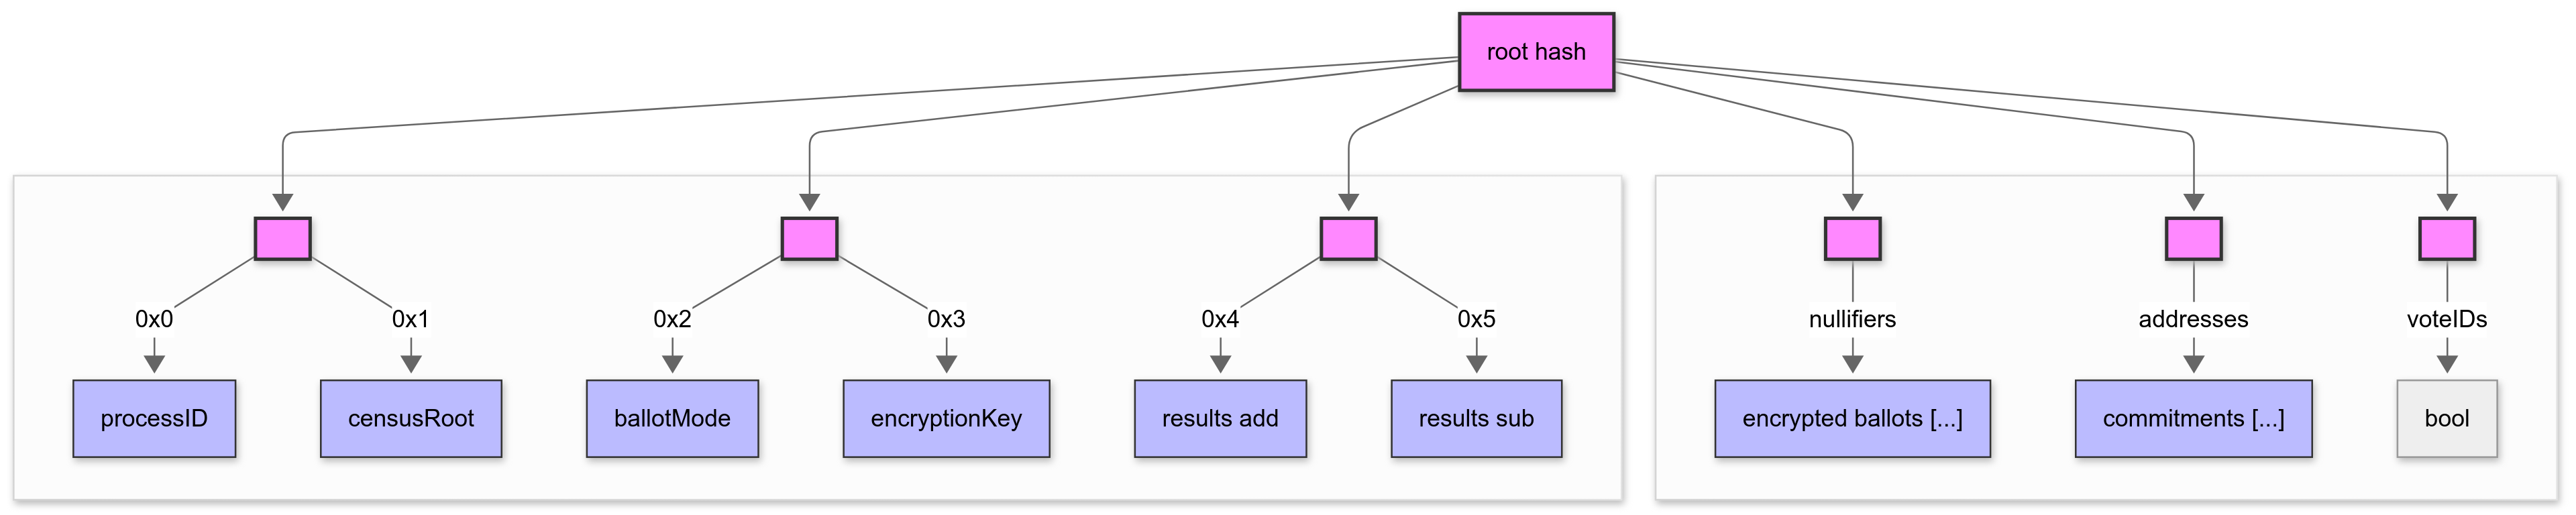
\includegraphics[width=400pt,draft=false]{\figs/mt-state-mermaid}}
	\caption{Structure of the state Merkle tree (FIGURE SHOULD BE POLISHED).}
	\label{fig:mt-state}
\end{figure}

\textbf{The Initial State}: The voting process begins with an initial state where the Merkle Tree Root is established and published on the Process Management smart contract. Predefined parameters are included, but the results are initialized to zero, and no nullifiers are present. The Process Organizer transaction, contains the initial root and the necessary Merkle proofs. These proofs verify that the initial parameters are correct according to the voting process information and that no additional information is stored. Since the `ProcessId` of the initial state is a unique identifier, there won't be duplicate roots for different processes.


\subsubsection{Smart contracts}

\paragraph{Process management.} This smart contract is responsible for the life-cycle management of voting processes. It includes the initiation, monitoring, execution, and closure of voting events.

\paragraph{Sequencer registry.} For each voting process, this smart contract maintains the integrity of the cast votes and process life cycle. It verifies that each state transition committed by a sequencer adheres to the predefined rules.

\paragraph{Results verification.} This smart contract keeps track of the existing available sequencers, stores the collateral of the sequencers to ensure (that incentivizes) good behaviour, and is used to coordinate the distributed key generation when a new voting process is created.\\

\martai{This is wrong. Explanation of SR and RV smart contracts are mixed, I don't know what I was thinking when I wrote it. We should also include a sentence about the management of sequencers.}


\begin{figure}[h]
	\centerline{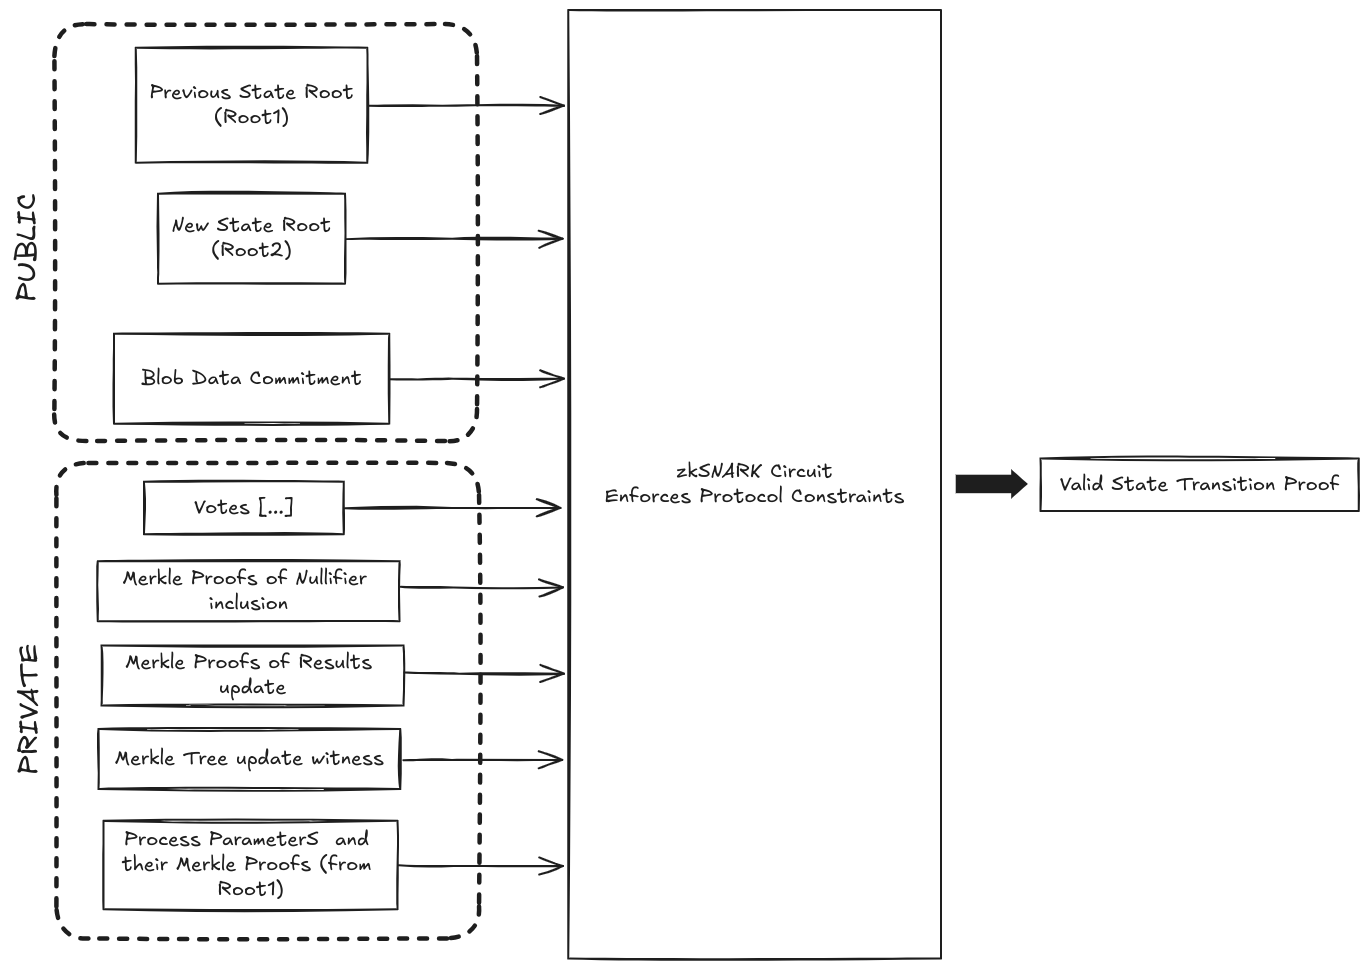
\includegraphics[width=400pt,draft=false]{\figs/circuit-inputs}}
	\caption{Caption.}
	\label{fig:circuit-inputs}
\end{figure}


\subsubsection{Votes [I don't think this is the right place]}

In the \davinci system, a vote comprises several components that work together to ensure secure, private, and verifiable voting. These components are:
\begin{align*}
		\vote = [	\processid, \voteid, \encryptedballot, \censuspf, \zkproof, \signature ].
\end{align*}
\martai{In the code, the struct is just: address, commitment, nullifier and ballot. Check!}

\martai{Actually, the address could be recomputed by the sequencer (add it as a footnote).}

\martai{In the code, they call it vote, verifierVote. Alternative: envelope.}

Below, we detail each component and its role in the voting process:
\begin{itemize}
	\item \processid: the process identifier is a unique 32-byte number that uniquely identifies a specific voting process. This variable encapsulates essential information about the voting, such as the rules and constraints for ballots and the unique identifier of the \davinci blockchain instance.
	\martai{the identifier is computed from the organization address, the Eth nonce, chain ID (e.g. mainnet), formatejat in a certain way.}
	%
	\item \encryptedballot: it contains the voter's selections encoded according to the ballot protocol rules. To ensure privacy, the ballot is encrypted using an homomorphic encryption scheme, which allows homomorphic combination of encrypted votes. More specifically, given the voter's choice $m$ and a random element $k$, the vote is encoded as follows:
	\[ \encryptedballot = \hlget{\Enc}(m; k). \]
	%
	\item \voteid: vote identifier, tied to balbla, computed this way.
	\[ \voteid = .\]
	%
	\item \censuspf: the census proof serves as the voter's identity verification mechanism, ensuring that only eligible voters can participate. Depending on the process configuration, the voter provides either a Merkle tree-based proof showing inclusion in the census true, or a credential issued by a trusted third party (e.g. from a credential service provider).
	%
	\item \zkproof: the voter generates a ZK proof to prove the correctness of the ballot and encryption process:
	\[ \zkproof = \text{Prove(), Circuit()}. \]
	This proof proves the correct computation of the vote encryption, the nullifier, the commitment, and the compliance with the ballot protocol rules.
	%
	\item \signature: the signature authenticates the vote and ensure that was cast by a legitimate voter. The voter signs necessary components using their private key, depending on the census configuration (e.g., ECDSA, EdDSA, RSA).	
	\[ \signature = \text{Sign(xxx)}. \]
\end{itemize}

\subsection{Circuits}
\label{sec:vocdoni-protocol:circuits}

\martai{The idea of this section is to describe the circuits. Then, in Section~\ref{sec:analysis:implementation} we give the details such as of the number of constants, framework used, etc. I haven't done this split yet.}

\martai{\textbf{About the circuits: in practice (and for optimization), all public inputs $PI$ are private, and we produce a single public input $h = Hash(PI)$. Then, the verifier checks that $Hash(PI) = h$ and verifies the proof only against $h$.} For this, we use the MiMC-7 hash function. Since this is an implementation detail, I propose to write this as a footnote or as an introduction to this section.}

\textit{Old text: By structuring the process this way, we ensure that voting can be performed from any device-including smartphones and web browsers-while keeping the sequencer's computational requirements within the capabilities of accessible, CPU-based machines with 64 GiB of memory.}

\martai{I don't follow the above paragraph.}

\martai{It is called Ballot Mode because we define some modes (like quadratic, etc.) that can be chosen by the organizer. Essentially, each of this modes has a special configuration, but in order to make it easier, the organizer only needs to choose which of the modes (configs) to apply.}

\martai{It's convenient to name the proof associated to each circuit: a proof for this circuit is called [...].\\
Answer: 1. ballotProof, 2. voteVerifier, 3. aggregator, 4. stateTransition.}

\begin{figure}[h]
	\centerline{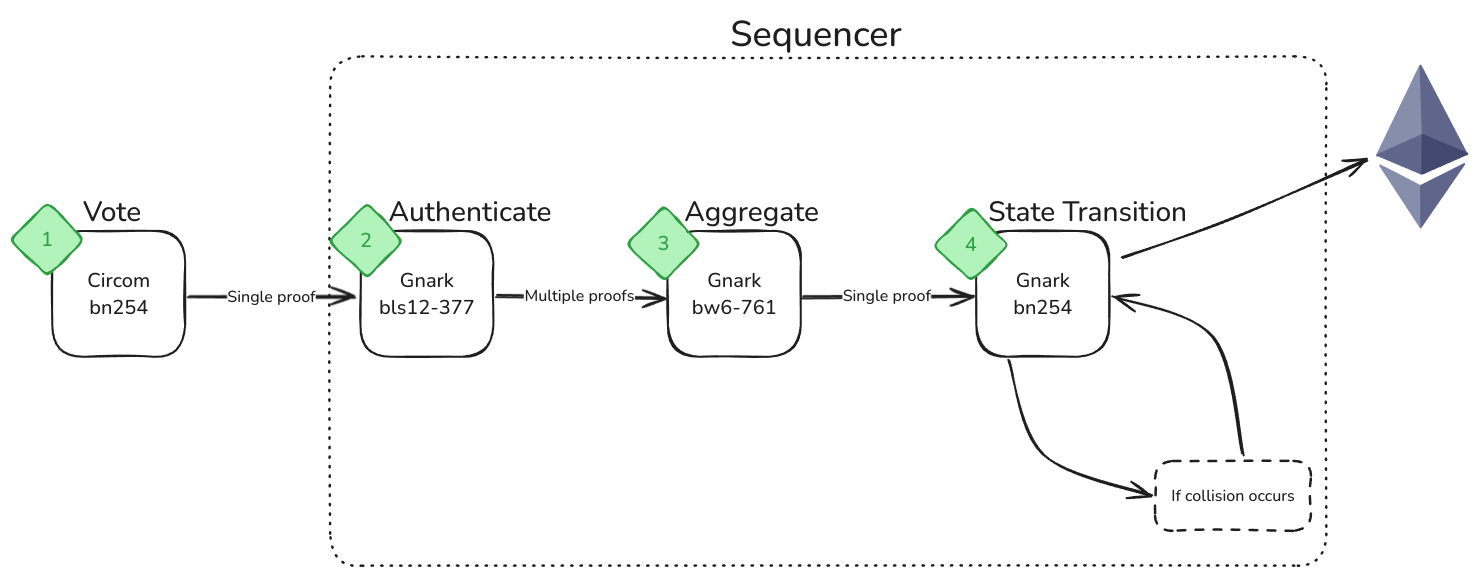
\includegraphics[width=350pt,draft=false]{\figs/circuits-flow}}
	\caption{Circuits flow.}
	\label{fig:circuits-flow}
\end{figure}

\pagebreak

\subsubsection{Voter circuit} 

Figure~\ref{fig:circuit-voter} -- BN254.\\

\noi Generated by the user when casting a vote, this circuit proves that the encrypted ballot is valid (i.e. follows the protocol rules) and that the vote identifier is correctly computed.

\begin{spacing}{1.25}
	\vspace{0.3cm}
	\noi \textbf{Public inputs}
	\begin{itemize}
		\item $\public$ $\processid$: voting process identifier. 
		\item $\public$ $\ballotmode$: ballot protocol configuration.S
		\item $\public$ $\epk$ ($EPK$): encryption public key.
		\item $\public$ $\address$: voter's address.
		\item $\public$ $\weight$: voter's weight.
		\item $\public$ $(C_1, C_2)$: encrypted ballot. 
		\item $\public$ $\voteid$: vote's unique identifier. 
	\end{itemize}
	\textbf{Private inputs}
	\begin{itemize}								
		\item \private $\ballot$: plaintext voter's voting choice.
		\item \private $k$: random scalar.
	\end{itemize}
	\textbf{Constraints}
	\begin{itemize}								
		\item \emph{Vote encryption}. Correct encryption of the ballot: $(C_1, C_2) = \hlget{\Enc}_{\epk}(\ballot, k).$
		\item \emph{Protocol rules compliance}. The ballot meets the protocol rules (number of valid choices, etc.): $... + \weight$.
		\item \emph{Vote identifier}. The vote's identifier is correctly computed: $\voteid = \text{Hash} (\address \conc \processid \conc k)$.
	\end{itemize}
	\vspace{-0.3cm}
\end{spacing}

\begin{figure}[H]
	\centerline{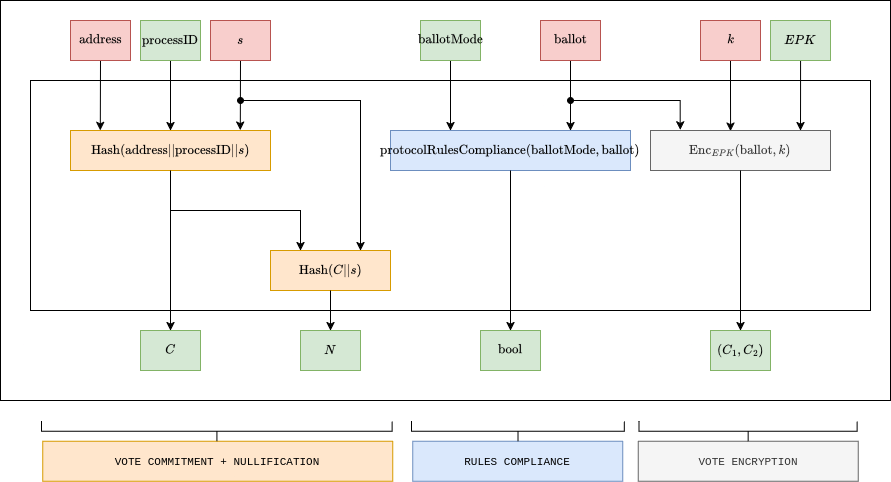
\includegraphics[width=450pt,draft=false]{\figs/circuit-voter}}
	\caption{Voter circuit. All public values are framed in green.}
	\label{fig:circuit-voter}
\end{figure}

\newpage
\subsubsection{Authentication circuit}
\label{sec:vocdoni-protocol:circuits:authentication}

Figure~\ref{fig:circuit-authentication} -- BLS12-377.\\

\noi Generated by the sequencer, this circuit transforms the vote proof to the BLS12-377 curve for native recursion and validates the user's eligibility in the census, as well as their signature.

\begin{spacing}{1.25}
	\vspace{0.3cm}
	\noi \textbf{Public inputs}
	\begin{itemize}
		\item \public $\voteproof$: voter's proof.
		\item \public $\processid$: process identifier.
		\item \public $\ballotmode$: ballot protocol configuration.
		\item \public $\epk$ ($EPK$): encryption public key.
		\item \public $(C_1, C_2)$: encrypted ballot.		
		\item \public $\voteid$: voter's identifier.
		\item \public $\weight$: voter's weight.
		\item \public $\censuspf$: census membership proof.
		\item \public $\censusroot$: census Merkle tree root.
		\item \public $\pk$: voter's public key.
		\item \public $\signature$: voter's signature.
	\end{itemize}
	\textbf{Constraints}	
	\begin{itemize}
		\item \emph{Voter's proof verification.} The vote zkProof is valid for the inputs provided: $P.Verify().$
		\item \emph{Census membership.} The address derived from the user's public key is part of the census, and verifies the census proof with the user's weight provided.
		\item \emph{Authentication + non-malleability.} The signature of the vote's identifier is valid for the given public key.
	\end{itemize}
	\vspace{-0.3cm}
\end{spacing}

\begin{figure}[H]
	\centerline{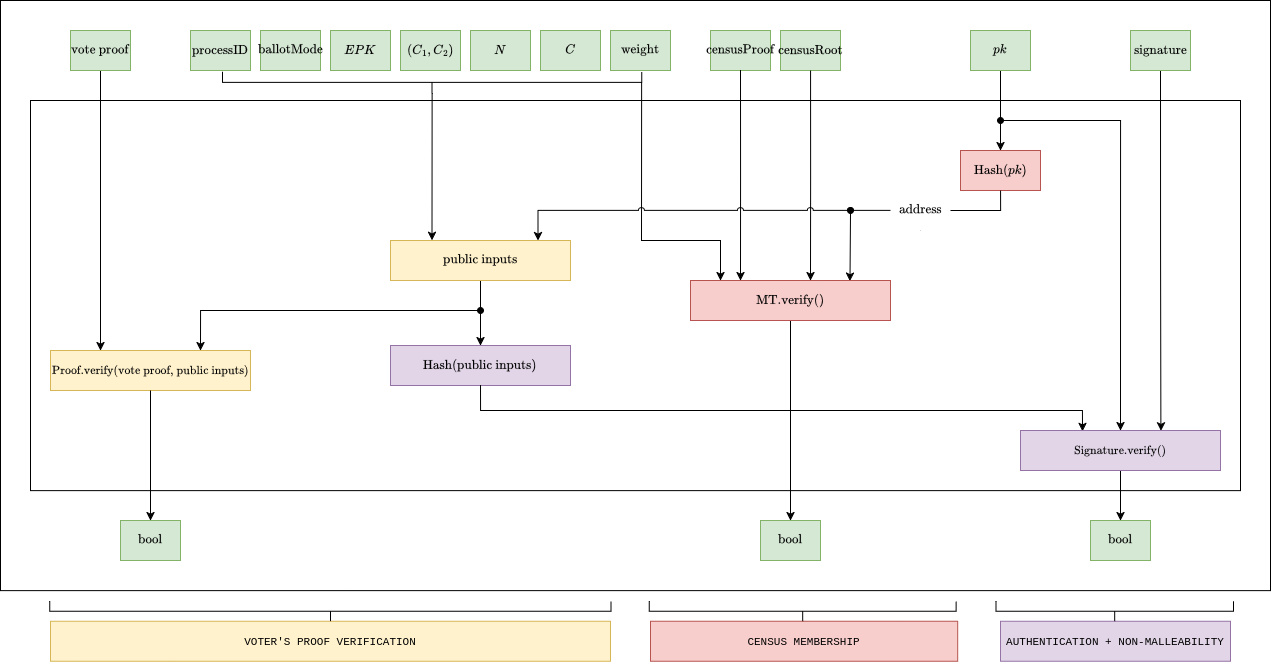
\includegraphics[width=450pt,draft=false]{\figs/circuit-authentication}}
	\caption{Authentication circuit. All public values are framed in green.}
	\label{fig:circuit-authentication}
\end{figure}

\newpage
\subsubsection{Aggregation circuit}

Figure~\ref{fig:circuit-aggregate} -- BW6-761.\\

\noi This circuit accumulates multiple authenticated votes into a single proof. It also verifies that all accumulated votes belong to the same voting process.

\martai{Actually, the circuit only takes voteProof and the hash(PI). Circuit 4 is the one that verifies shared PI.}

\martai{The batch, number of verification proofs, is a fixed parameter (currently set to 60). If it includes less proofs than the max size of the batch, the sequencer adds dummy proofs to the circuit.}

\begin{spacing}{1.25}
	\vspace{0.3cm}
	\noi \textbf{Public inputs}
	\begin{itemize}
		\item \public $\text{authenticationProof}_i$: set of authentication proofs.
		\item \public $\text{voteProof}_i$: set of authentication proofs.
		\item \public $(C_1, C_2)$: list of voters' encrypted ballots.
		\item \public $\voteid_i$: set of vote's identifiers.
		\item \public $\pk_i$: list of voters' public keys.
		\item \public $\weight_i$: Voters' weights.
		\item \public $\text{censusProof}_i$: Voters' weights.
		\item \public $\signature_i$: Voters' weights.
		\item \public $\processid$: process identifier.
		\item \public $\ballotmode$: ballot protocol configuration.
		\item \public $EPK$: encryption public key.
		\item \public $\censusroot$: census Merkle tree root.
	\end{itemize}
	\textbf{Constraints} \\ \vspace{-0.4cm}		
	\begin{itemize}
		\item \emph{Votes aggregation.} The accumulated authentication zkProofs are valid (for the given inputs).
		\item \emph{Shared public inputs.} The \processid, \censusroot, \ballotmode and $EPK$ are the same for all of them.
	\end{itemize}
	\vspace{-0.3cm}
\end{spacing}

\begin{figure}[h]
	\centerline{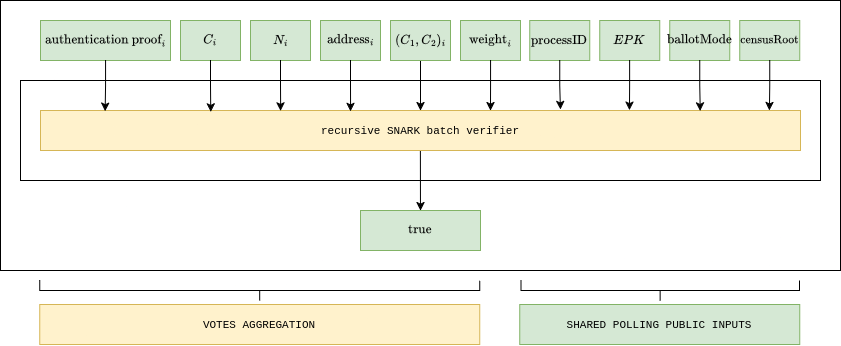
\includegraphics[width=450pt,draft=false]{\figs/circuit-aggregate}}
	\caption{Aggregation circuit. All public values are framed in green.}
	\label{fig:circuit-aggregate}
\end{figure}

\newpage
\subsubsection{State transition circuit} -- BN254. \\

\noi Given the aggregated votes proof, this circuit verifies the correct inclusion of all new votes into the process's state Merkle tree. It generates the final state transition proof that will be validated by the Ethereum smart contract.

\paragraph{Assertions.}

\begin{itemize}
	\item \emph{Aggregation verification}: The agreggated zkProof is valid.
	\item \emph{Transition verification}: The MerkleTree transition witness proves every change between Root1 and Root2.
	\item \emph{Public inputs integrity}: ProcessID, BallotMode, CensusRoot, EncryptionKey remain unchanged.
	\item \emph{Votes counting}: Ballots are correctly counted as new or overwrites, and added to results accumulators.
\end{itemize}

\martai{The corresponding circuit figure is not done yet.}

\noi \textit{Old original text, I think it will help here:}

When a new voting process begins, the Sequencer initializes a new State, represented by the root hash of a Merkle tree. This tree encapsulates all essential information about the voting process, including process parameters, voter registry (census), ballot configurations, and initial results.

For each new batch of votes, the Sequencer updates the state by generating a zkSNARK proof that \textbf{validates the state transition from the current Root to a new Root}. This proof is submitted on-chain for settlement. By doing so, we maintain an immutable and verifiable record of the voting process on the blockchain.

This approach allows anyone to access the latest verified state of the voting process from the Results Verification smart contract, along with the necessary data to process subsequent state updates. The system's design enables multiple Sequencers to participate in tallying votes. They can take the current State Root and its associated data to construct the next state, incorporating new votes into the tally. This decentralization of Sequencers helps prevent potential censorship and reinforces the robustness of the voting process.

\paragraph{Maintaining the Chain.}

The chain of integrity is maintained through a combination of smart contract enforcement and strict zkSNARK circuit constraints. This ensures that each state transition is valid and builds upon the last accepted state without requiring additional mechanisms.

\begin{itemize}
	\item \textbf{Sequential state roots}: Each state transition updates the Merkle tree from a previous root (`Root1`) to a new root (`Root2`) after processing a batch of votes.
	\item \textbf{Smart contract enforcement}: The smart contract verifies that the `Root1` provided in the zkSNARK proof matches the last committed state root stored on-chain. This guarantees that all transitions are sequential and based on the latest accepted state.
	\item \textbf{Proof validation}: The smart contract uses the zkSNARK verification key to validate the submitted proof. A valid proof confirms that the transition from `Root1` to `Root2` adheres to all protocol rules enforced by the circuit.
	\item \textbf{State update}: Upon successful verification, the smart contract updates the stored state root hash to`Root2`, ensuring an immutable and continuous chain of states.
\end{itemize}

\paragraph{State Transition}

To validate and process state transitions, \textbf{we employ a zkSNARK circuit that enforces all protocol constraints}. This circuit proves that the transition from the previous state Root to the new state Root is valid based on the newly processed votes.

\begin{figure}[H]
	\centering
	\fbox{
		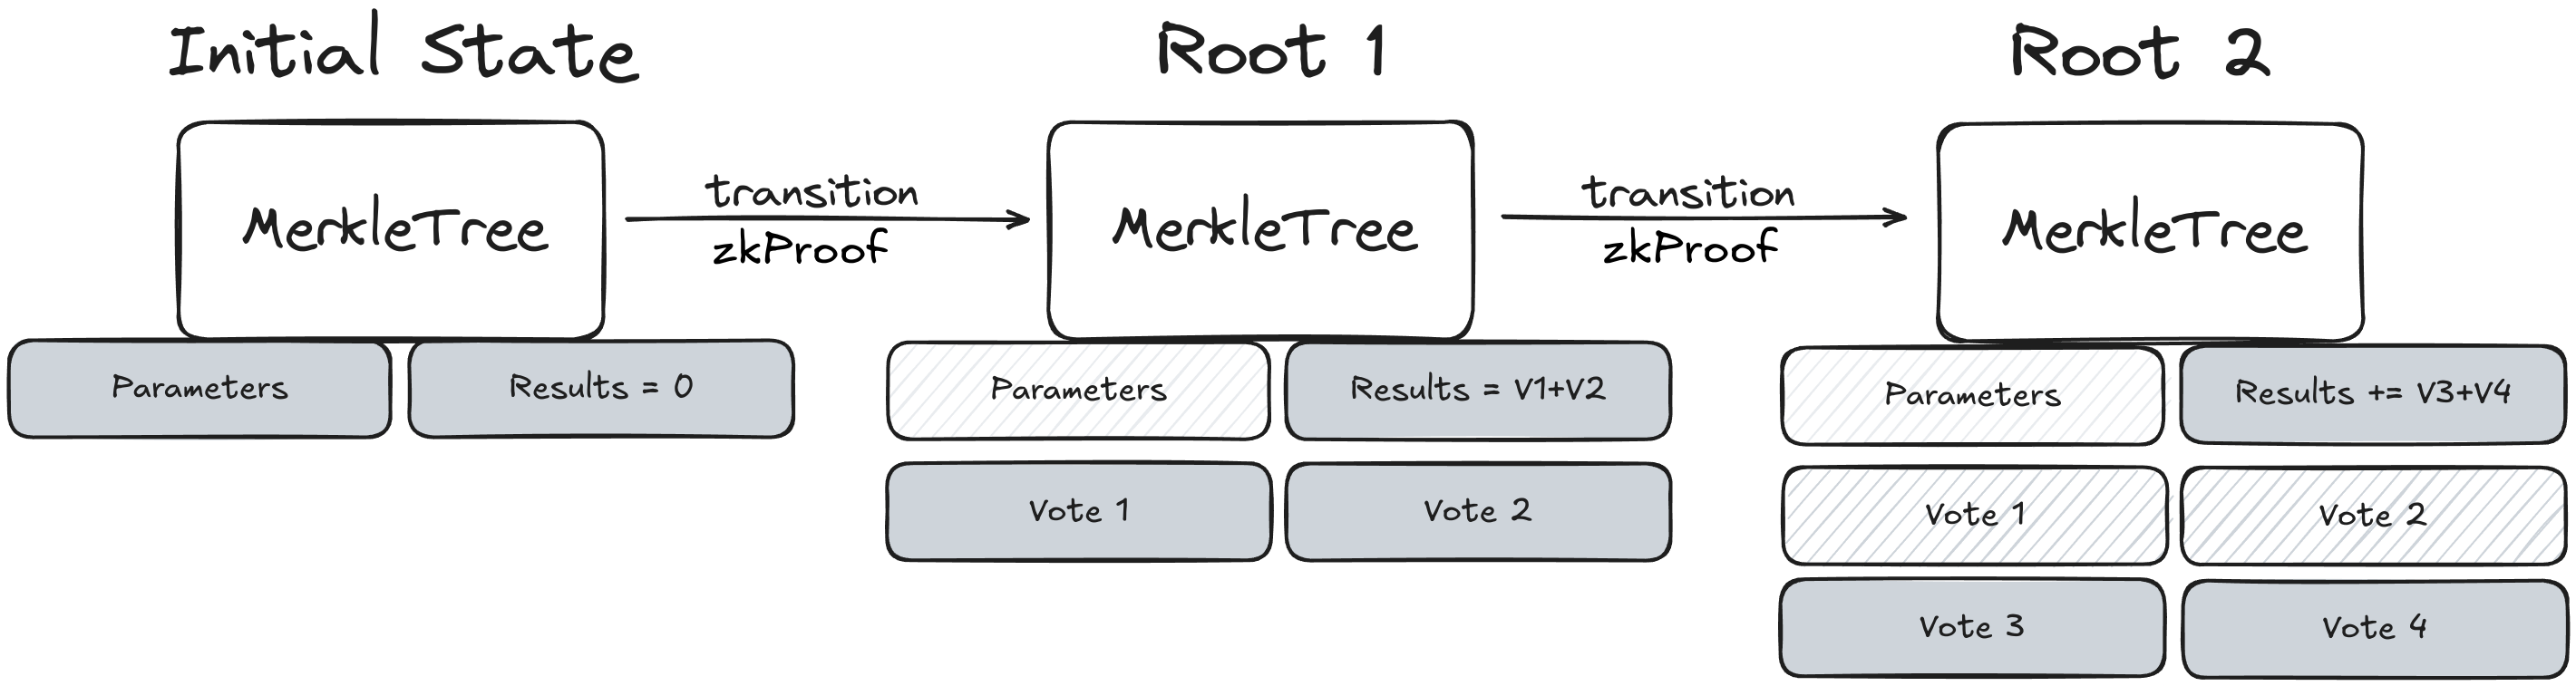
\includegraphics[scale = 0.12, draft = false]{\figs/state-transition.png}}
\end{figure}

\begin{figure}[H]
	\centering
	\fbox{
		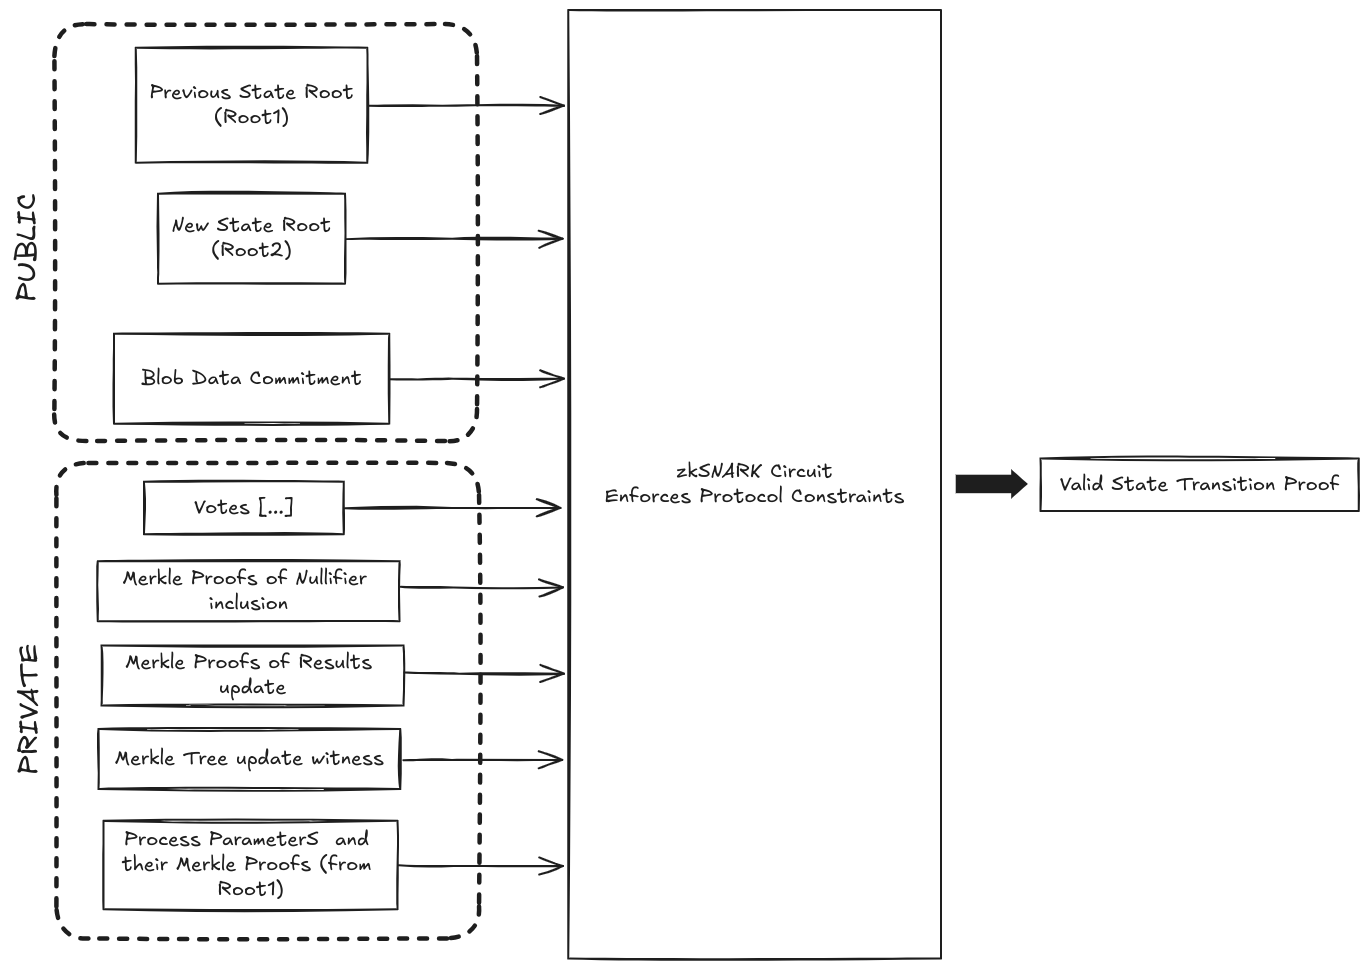
\includegraphics[scale = 0.3, draft = false]{\figs/circuit-inputs.png}}
\end{figure}

\begin{figure}[H]
	\centerline{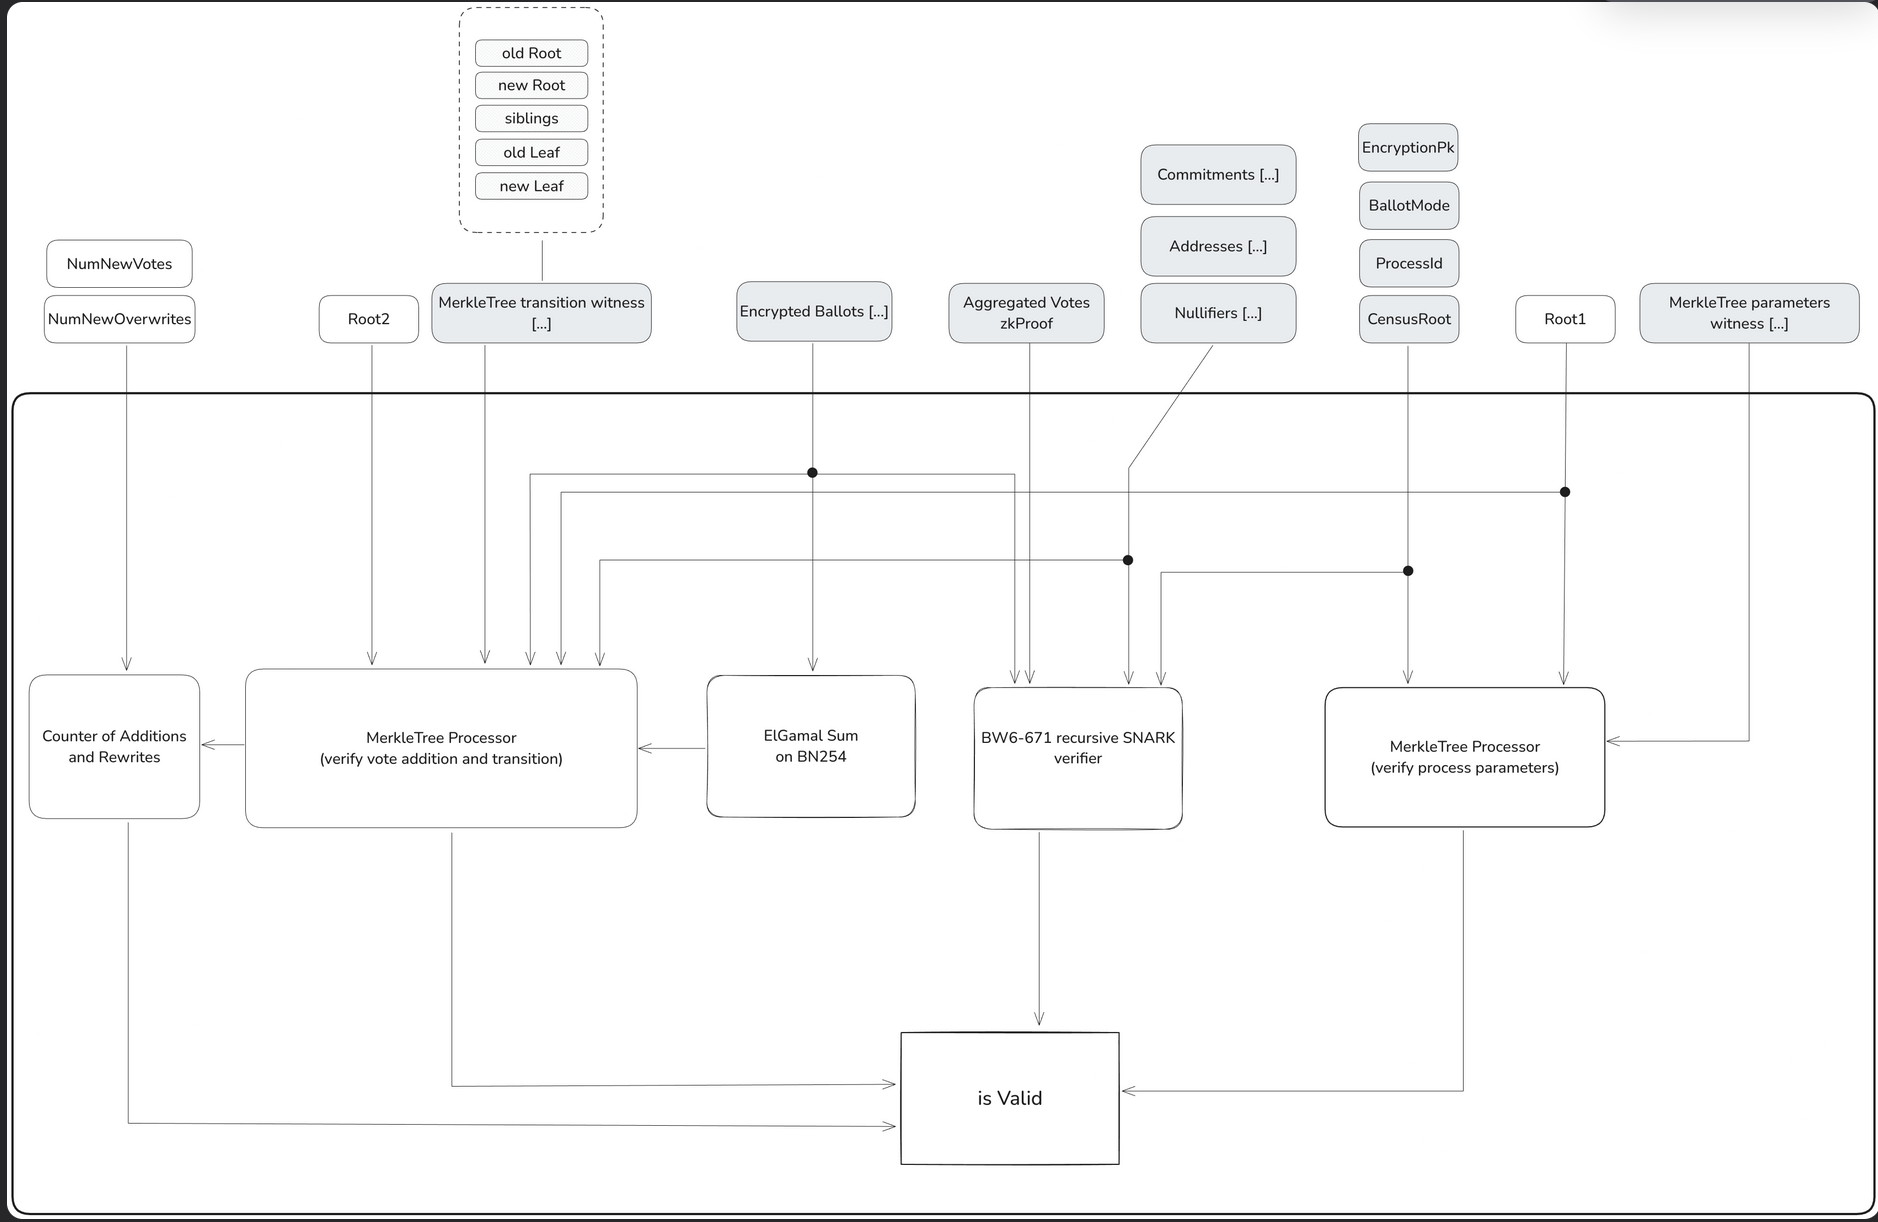
\includegraphics[width=400pt,draft=false]{\figs/circuit-state-transition}}
	\caption{State transition circuit. All public values are framed in green.}
	\label{fig:circuit-state-transition}
\end{figure}

\begin{mdframed}
	\begin{minipage}[H]{1\textwidth}
		\begin{spacing}{1.25}
			\vspace{0.3cm}
			\begin{center}{STATE TRANSITION CIRCUIT}\end{center}
			\textbf{Public inputs}
			\begin{itemize}
				\item \public $root_{old}$: Merkle tree root before the state transition.
				\item \public $root_{new}$: Meklre tree root after the state transition.
				\item \public $blobCommitment$: the commitment to the data blob containing the new votes.
				\end{itemize}
				\item \textbf{Private inputs}
				\begin{itemize}
				\item \private Votes: The list of new votes being processed, including census proofs and authentication data.
				\item \private Merkle Proofs of nullifier inclusion: Proofs that each voter nullifier is included in the census.
				\item \private Merkle Proofs of results update: Proofs that the process results have been correctly updated.
				\item \private Merkle Tree Update Witnesses: Necessary data (e.g., Merkle paths) to update the Merkle tree from Root1 to Root2.
				\item \private Process Parameters: Retrieved from Root1 within the circuit.
			\end{itemize}
			\textbf{Constraints} \\ \vspace{-0.4cm}		
			\begin{itemize}
				\item \textbf{Immutable process parameters}: Ensure that critical process parameters (such as `censusRoot` or `processId`) retrieved from `Root1` remain consistent and are not altered in the transition.
				\item \textbf{Vote validity}: Validate that each vote proof is correct.
				\item \textbf{Voter eligibility}: Confirm that each voter is included in the census by verifying Merkle proofs of inclusion against the `censusRoot` retrieved from `Root1`.
				\item \textbf{Nullifier non-existence}: Ensure that the nullifier for each vote does not exist in the current state (`Root1`), preventing double voting.
				\item \textbf{Nullifier addition}: Correctly add each new nullifier to the state, resulting in `Root2`, updating the Merkle tree accordingly.
				\item \textbf{Results update}: Ensure that the voting results are accurately updated by adding the new votes to the previous results retrieved from `Root1`, so that `results2 = results1 + votes`.
				\item \textbf{Blob data integrity}: Confirm that the data used in the circuit (votes, nullifiers) corresponds to the `blobCommitment` provided as a public input, ensuring that the votes processed are exactly those published in the data blob.
				\item \textbf{State transition validity}: Ensure that the new state root (`Root2`) is correctly computed from `Root1` by applying the validated votes and updates to the Merkle tree.
			\end{itemize}
			\vspace{-0.3cm}
		\end{spacing}
	\end{minipage}
\end{mdframed}

\martai{STATE TRANSITION CIRCUIT: a potential problem is that a sequencer may know if one of their votes has been overwritten, for this reason, sequencers reencrypt a certain amount of ballots every time (already existing ballots I mean). So, the circuit should include the reencryptions: both for existing ballots and also for the new votes, which should be reencrypted (for receipt-freeness).}

\subsection{Protocol flow}
\label{sec:vocdoni-protocol:flow}

In Figure~\ref{fig:protocol-flow} we describe the protocol flow.

\martai{About the figure: layout should be fixed. In addition, the icons for the different parties are missing.}

\begin{figure}[H]
	\centerline{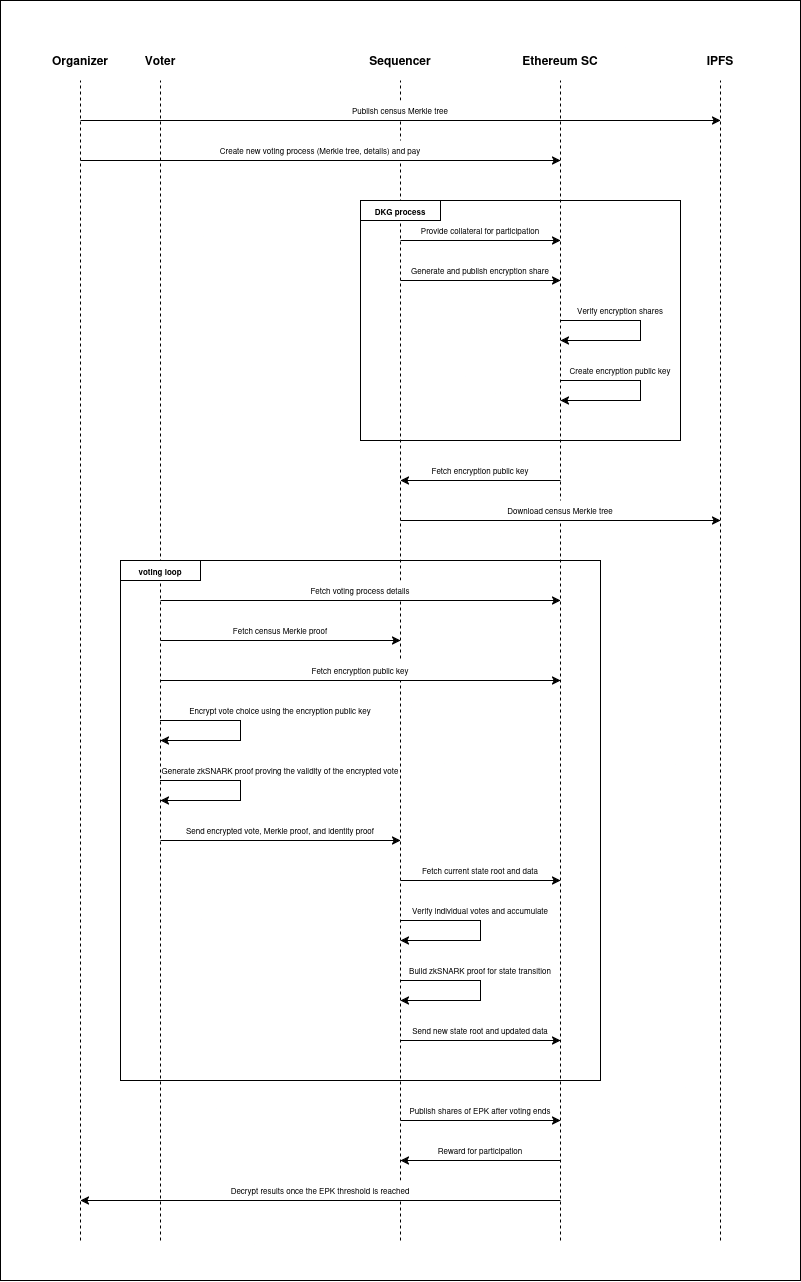
\includegraphics[width=400pt,draft=false]{\figs/protocol-flow}}
	\caption{Vocdoni voting process overview.}
	\label{fig:protocol-flow}
\end{figure}

\subsubsection{Prior to voting (only once)}
\label{sec:vocdoni-protocol:prior-steps}

\martai{Remove the first step, we assume contracts are already deployed or at least, the logic is available.}

This is done only once. Then every voting will start its process from step in Section~\ref{sec:vocdoni-protocol:start}.

Vocdoni:
\begin{enumerate}
	\item Deployment of the 3 smart contracts.
	\item Sequencers registry starts (it doesn't end).
\end{enumerate}

Sequencers (nodes validadors) -- this process is always open:
\begin{enumerate}
	\item Register this and that way.
	\item Public keys?
	\martai{Sequencers must also publish how they can be reached (either when they register or when they contribute to the DKG). They can use a URI: Uniform Resource Identifier.}
	\item PROVIDE COLLATERAL.
	\martai{What happens to the collateral? If done only once, then you lose it? Do you need to send a new tx with more collateral?}
	\item Send transaction to Sequencer registry smart contract (pay for tx fee).
\end{enumerate}

\subsubsection{Start of the voting process}
\label{sec:vocdoni-protocol:start}

The organizer:
\begin{enumerate}
	\item Prepares the census data \texttt{census\_data}.
	\item Generates the census commitment \texttt{MT\_census.root = Com(census\_data)}.
	\martai{In general, make use (link) to the functions defined in Section~\ref{sec:cryptographic-primitives}. For example, here the \texttt{MT.root()}.}
	\martai{Additionally, after this step, the organizer should make a Merkle proof available to all eligible voters.}
	\item Set voting details: duration, options, type, etc. + CENSUS MT ROOT.
	\item Also a timeout for the DKG ceremony + minimum number of sequencers.
	\item Send transaction to the Ethereum process management smart contract with all data. Note this transaction has a cost (Eth tx fees) that needs to be covered by the organizer.
\end{enumerate}

\subsubsection{Encryption key generation process} %Voting key generation
\label{sec:vocdoni-protocol:dkg}

The sequencer:
\begin{enumerate}
	\item Download all required data from the PM smart contract which includes the census MT root to handle the new vote.
	\item Make contributions to DKG ceremony.
\end{enumerate}

After XXX time (set by the organizer in the PM contract?): all contributions to DKG are done.

\martai{The organizer decides a minimum number of sequencers (security factor).}
	
\begin{itemize}
	\item EPK ``becomes available".
	\martai{I understand EPK becomes available in the SR smart contract, and that key is sent to the PM contract?}
	\martai{The idea here is that some sequencer makes EPK available (a.k.a. sends a transaction). Alternatively, generate a SNARK proving the EPK has been generated correctly and the SC verifies it.}
\end{itemize}

\subsubsection{Voting process}
\label{sec:vocdoni-protocol:voting}

Voter:

\begin{itemize}
	\item Choose any of the available sequencers (from?? -- from the SR SC).
	\item Fetch their census \textbf{Merkle proof} to prove eligibility (from the census registry).
	\item Use the EPK to encrypt the voting choice.
	\item Generate ZK-SNARK of satisfiability of circuit from Fig.~\ref{fig:circuit-voter} with protocol from Section~\ref{sec:cryptographic-primitives:zkp} to prove the validity of the encrypted vote and adherence to ballot protocol rules. We call this proof \textbf{vote proof}.
	\item Send the encrypted vote, Merkle proof, validity proof, and identity proof to the sequencer.
	\martai{I understand Validity proof refers to ``voter circuit"? Merkle proof is for inclusion, right? And identity proof is for example a signature??}
\end{itemize}

Sequencer:

\begin{itemize}
	\item Fetch current state: retrieve the current valid process state root from the Etherem smart contract and the associated data from Ethereum blobs.
	\martai{specify which SC.}
	\item Generate a SK-SNARK proof of state transition proving:
		\begin{itemize}
			\item the validity of the ZK-SNARK proof provided by the voter,
			\item the correct accumulation of votes from users, adding them to the process state,
			\item the correct sum of the new encrypted votes using the homomorphic properties of ElGamal,
			\item the new votes are from eligible users by checking the census Merkle proofs,
			\item the new voters have not already voted by checking their nullifiers, or it is a correct vote overwrite,
			\item the data blob hash matches the data used to verify the transition.
		\end{itemize}
	\item Submit updated state: send the new state root to the smart contract and store the updated data in Ethereum blobs.
\end{itemize}

Sequencers keep accumulating votes and create state transition until the finalization of the process.

\martai{I understand this finalization is a deadline set by the organizer.}

SC:

\begin{itemize}
	\item Upon receiving a sequencer's transaction, the SC verifies the zk-SNARK proof provided byt he sequencer.
	\item Ensure the origin root corresponds to the current stored state root.
	\item Confirm that the blob hash matches the one stored in Ethereum.
\end{itemize}

\subsubsection{Results validation}
\label{sec:vocdoni-protocol:validation}

Once the voting is completed (I understand the timeout set by the organizer expires), the following things happen.

Sequencer:

\begin{itemize}
	\item $t$ out of $n$ sequencers publish their shares corresponding to the EPK to the Ethereum smart contract.
	\martai{specify which SC.}
	\item When the threshold of shares is reached, the results can be decrypted by anyone.
	\martai{mention that the SC computes the corresponding ESK, or that can be computed by anyone off-chain, since all info is public.}
	\item Sequencers receive reward for their correct participants depending on the number of sequenced votes.
	\martai{slash if they don't provide the right share? reward only dependent of sequenced votes? any relation to their participation in the computation of either EPK or ESK?}
\end{itemize}

This way:

\begin{itemize}
	\item After the voting period ends and the results are decrypted, anyone can verify the correctness of the final result.
	\martai{explain how.}
	\item Use the zkSNARK state proof and publicly available data on-chain to ensure the integrity and correctness of the entire voting process.
	\martai{elaborate on this.}
\end{itemize}

\subsubsection{Finalization of the voting process}
\label{sec:vocdoni-protocol:finalization}
